% ! TeX program = lualatex
\documentclass[a4paper,11pt]{article} 
% packages
\usepackage{censor}
\StopCensoring
\usepackage{fontspec}
\setmainfont{EB Garamond}
% for tironian et fallback
% % \directlua{luaotfload.add_fallback
% % ("emojifallback",
% %      {"Noto Serif:mode=harf"}
% % )}
% % \setmainfont{EB Garamond}[RawFeature={fallback=emojifallback}]

\setmonofont[Scale=MatchLowercase]{Deja Vu Sans Mono}
\usepackage[a4paper,left=2cm,right=2cm,top=\dimexpr15mm+1.5\baselineskip,bottom=2cm]{geometry}
\setlength{\parindent}{0pt}

\usepackage{fancyhdr}       % Headers and footers 
\fancyhead[R]{\normalfont \leftmark}
\fancyhead[L]{}
\pagestyle{fancy}

\usepackage{microtype}      % Slightly tweak font spacing for aesthetics
\usepackage[english]{babel} % Language hyphenation and typographical rules
\usepackage{xcolor}
\definecolor{linkblue}{RGB}{0, 64, 128}
\usepackage[final, colorlinks = false, urlcolor = linkblue]{hyperref} 
% \newcommand{\secref}[1]{\textbf{§~\nameref{#1}}}
\newcommand{\secref}[1]{\textbf{§\ref{#1}~\nameref{#1}}}

\usepackage{changepage}     % adjust margins on the fly
\usepackage{amsmath,amssymb}

\usepackage{minted}
\usemintedstyle{algol_nu}

\usepackage{pgfplots}
\pgfplotsset{width=\textwidth,compat=1.9}

\usepackage{caption}
\newenvironment{code}{\captionsetup{type=listing}}{}
\captionsetup[listing]{skip=0pt}
\setlength{\abovecaptionskip}{5pt}
\setlength{\belowcaptionskip}{5pt}

\usepackage[yyyymmdd]{datetime}
\renewcommand{\dateseparator}{--}

\usepackage{enumitem}

\usepackage{titlesec}

\author{Andrew Hayes}

\begin{document}
\begin{titlepage}
    \begin{center}
        \hrule
        \vspace*{0.6cm}
        \Huge \textsc{ct414}
        \vspace*{0.6cm}
        \hrule
        \LARGE
       \vspace{0.5cm}
       Distributed Systems \& Co-Operative Computing
       \vspace{0.5cm}
       \hrule

       \vfill

       \hrule
        \begin{minipage}{0.495\textwidth} 
            \vspace{0.4em}
            \raggedright
            \normalsize 
            \begin{tabular}{@{}l l}
                Name: & Andrew Hayes \\
                Student ID: & 21321503 \\
                E-mail: & \href{mailto://a.hayes18@universityofgalway.ie}{a.hayes18@universityofgalway.ie} \\
            \end{tabular}
        \end{minipage}
        \begin{minipage}{0.495\textwidth} 
            \raggedleft
            \vspace*{0.8cm}
            \Large
            \today
            \vspace*{0.6cm}
        \end{minipage}
        \medskip\hrule 
    \end{center}
\end{titlepage}

\pagenumbering{roman}
\newpage
\tableofcontents
\newpage
\setcounter{page}{1}
\pagenumbering{arabic}

\section{Introduction}
\subsection{Client-Server Architectures}
\subsubsection{Two-Tier Architectures}
A \textbf{two-tier client-server architecture} is a client-server architecture wherein a client talks directly to a server, with no intervening server.
It is typically used in small environments ($\lesssim$ 50 users).
\\\\
A common development error is to prototype an application in a small, two-tier environment, and then scale up by simply adding more users to the server:
this approach will usually result in an ineffective system, as the server becomes overwhelmed.
To properly scale to hundreds or thousands of users, it is usually necessary to move to a three-tier architecture.

\begin{figure}[H]
    \centering
    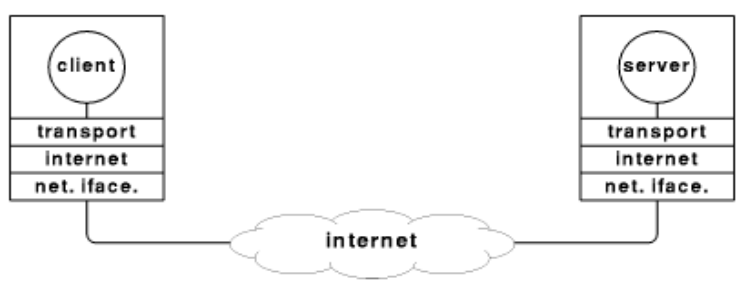
\includegraphics[width=0.7\textwidth]{./images/client-server-tcpip.png}
    \caption{
        Client \& server using TCP/IP protocols to communicate.
        Information can flow in either or both directions.
        The client \& server can interact with a transport layer protocols.
    }
\end{figure}

\subsection{Three-Tier Architecture}
A \textbf{three-tier client-server architecture} introduces a server or \textbf{agent} (or \textbf{load-balancer}) between the client \& the server.
The agent has many roles:
\begin{itemize}
    \item   Translation services: such as adapting a legacy application on a mainframe to a client-server environment.
    \item   Metering services: such as acting as a transaction monitor to limit the number of simultaneous requests to a given server.
    \item   Intelligent agent services: as in mapping a request to a number of different servers, collating the results, and returning a single response to the client.
\end{itemize}

\subsection{Network Programming Paradigms}
Practically all network programming is based on a client-server model; the only real difference in paradigms is the \textbf{level} at which the programmer operates.
The sockets API provides direct access to the available transport layer protocols.
RPC is a higher-level abstraction that hides some of the lower-level complexities.
Other approaches are also possible:
\begin{itemize}
    \item   Sockets are probably the best-known and most widely-used paradigm.
            However, problems of data incompatibility across platforms can arise.

    \item   RPC libraries aim to solve some of the basic problems with sockets and provide a level of transport independence.

    \item   Neither approach works very well with modern applications (Java RMI and other mdoern technologies, e.g., web services are better).
\end{itemize}

\section{Java RMI}
\textbf{Remote Method Invocation (RMI)} is a Java-based mechanism for distributed object computing.
RMI enables the distribution of work to other Java objects residing in other processes or on other machines.
The objects in one Java Virtual Machine (JVM) are allowed to seamlessly invoke methods on objects in a remote JVM.
To call a method of a remote object, we must first get a reference to that object, which can be obtained from  the registry name facility or by receiving the reference as an argument or return value of a method call.
Clients can call a remote object in a server that itself is a client of another server.
Parameters of method calls are passed as serialised objects: 
\begin{itemize}
    \item   types are not truncated, and therefore, object-oriented polymorphism is supported;
    \item   parameters are passed by value (deep copy) and therefore object behaviour can be passed.
\end{itemize}

The Java Object Model is still supported with distributed (remote) objects.
A reference to a remote object can be passed to or returned from local \& remote objects.
Remote object references are passed by reference: therefore, the whole object is not always downloaded.
Objects that implement the \mintinline{java}{Remote} interface are passed as a remote reference, while other objects are passed by value (using object serialisation).

\begin{figure}[H]
    \centering
    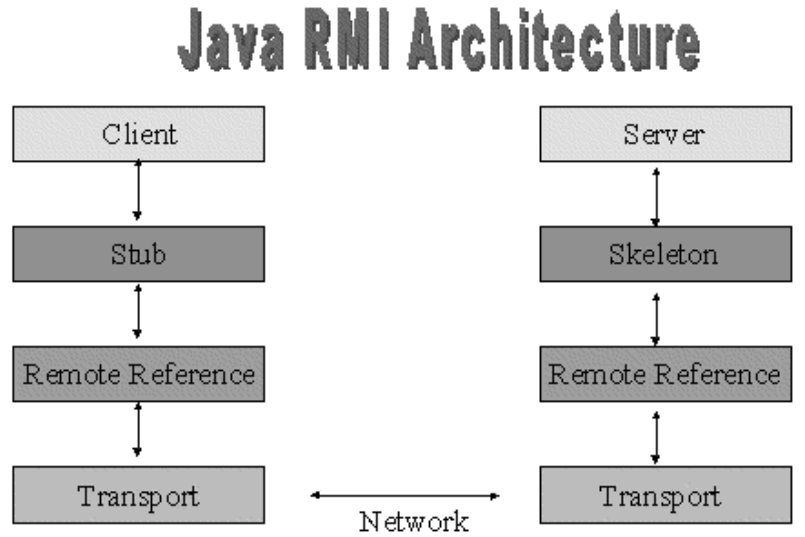
\includegraphics[width=0.8\textwidth]{./images/javarmi.png}
    \caption{Java RMI Architecture}
\end{figure}

The client obtains a reference for a remote object by calling \mintinline{java}{Naming.lookup(//URL/registered_name)} which is a method which returns a reference to another remote object.
Methods of the remote object may then be called by the client.
This call is actually to the \textbf{stub} which represents the remote object.
The stub packages the arguments (\textbf{marshalling}) into a data stream (to be sent across the network).
On the implementation side, the skeleton unmarshals the argument, calls the method, marshals the return value, and sends it back.
The stub unmarshals the return value and returns it to the caller.
The RMI layer sits on top of the JVM and this allows it to use Java Garbage Collection of remote objects, Java Security (a security manager may be set for the server, now deprecated), and Java class loading.

\subsection{Steps to Creating an RMI Application}
\begin{enumerate}
    \item   Define the interfaces to your remote objects.
    \item   Implement the remote object classes.
    \item   Write the main client \& server programs.
    \item   Create the stub \& skeleton classes by running the \textit{rmic} compiler on the remote implementation classes. (No longer needed in later Java versions).
    \item   Start the \textit{rmiregistry} (if not already started).
    \item   Start the server application.
    \item   Start the client (which contains some initial object references).
    \item   The client application/applet may then call object methods in the remote (server) program.
\end{enumerate}

\subsection{Example Java RMI Program}
\begin{code}
\begin{minted}[linenos, breaklines, frame=single]{java}
// Remote Object has a single method that is passed
// the name of a country and returns the capital city.
import java.rmi.*;

public interface CityServer extends Remote
{
    String getCapital(String Country) throws
        RemoteException;
}
\end{minted}
\caption{Example Java RMI Program}
\end{code}

\begin{code}
\begin{minted}[linenos, breaklines, frame=single]{java}
import java.rmi.*;
import java.rmi.server.*;

public class CityServerImpl
    extends UnicastRemoteObject
    implements CityServer
{
    // constructor is required in RMI
    CityServerImpl() throws RemoteException
    {
        super(); // call the parent constructor
    }

    // Remote method we are implementing!
    public String getCapital(String country) throws
        RemoteException
    {
        System.out.println("Sending return string now - country requested: " + country);
        if (country.toLowerCase().compareTo("usa") == 0)
            return "Washington";
        else if (country.toLowerCase().compareTo("ireland") == 0)
            return "Dublin";
        else if (country.toLowerCase().compareTo("france") == 0)
            return "Paris";
        return "Don't know that one!";
    }

    // main is required because the server is standalone
    public static void main(String args[])
    {
        try
        {
            // First reset our Security manager
            System.setSecurityManager(new RMISecurityManager());
            System.out.println("Security manager set");

            // Create an instance of the local object
            CityServerImpl cityServer = new CityServerImpl();
            System.out.println("Instance of City Server created");

            // Put the server object into the Registry
            Naming.rebind("Capitals", cityServer);
            System.out.println("Name rebind completed");
            System.out.println("Server ready for requests!");
        } catch(Exception exc)
        {
            System.out.println("Error in main - " + exc.toString());
        }
    }
}
\end{minted}
\caption{Example Server Implementation}
\end{code}

\begin{code}
\begin{minted}[linenos, breaklines, frame=single]{java}
public class CityClient
{
    public static void main (String args[])
    {
        CityServer cities = (CityServer) Naming.lookup("//localhost/Capitals");
        try {
            String capital = cities.getCapital("USA");
            System.out.println(capital);
        } catch (Exception e) {}
    }
}
\end{minted}
\caption{Example Client Implementation}
\end{code}

No distributed system can mask communication failures: method semantics should include failure possibilities.
Every RMI remote method must declare the exception \mintinline{java}{RemoteException} in its \mintinline{java}{throw} clause.
This exception is thrown when method invocation or return fails.
The Java compiler requires the failures to be handled.
\\\\
When implementing a remote object, the implementation class usually extends the RMI class \mintinline{java}{UnicastRemoteObject}: this indicates that the implementation class is used to create a single (non-replicated) remote object that uses RMI's default sockets-based transport for communication.
If you choose to extend a remote object from a non-remote class, you need to explicitly export the remote object by calling the method \mintinline{java}{UnicastRemoteObject.exportObject()}.
\\\\
The main method of the service first needs to create \& install a \textbf{security manager}, either the \mintinline{java}{RMISecurityManager} or one that you have defined yourself.
A security manager needs to be running so that it can guarantee that the classes loaded do not perform ``sensitive'' operations.
If no security manager is specified, no class loading for RMI classes is allowed, local or otherwise.
\\\\
TO make classes available via a web server (or your classpath), copy them into your public HTML directory.
Alternatively, you could have compiled your files directly into your public HTML directory:
\begin{minted}[linenos, breaklines, frame=single]{shell}
javac -d ~/project_dir/public_html City*.java
rmic -d ~/project_dir/public_html  CityServerImpl
\end{minted}

The files generated by \mintinline{shell}{rmic} (in this case) are: \verb|CityServerImpl_Stub.class| \& \verb|CityServerImpl_Skel.class|.
\\\\
\textbf{Polymorphic distributed computing} is the ability to recognise (at runtime) the actual implementation type of a particular interface.
We will use the example of a remote object that is used to computer arbitrary tasks:
\begin{itemize}
    \item   Client sends task object to compute server.
    \item   Compute server runs task and returns result.
    \item   RMI loads task code dynamically in the server.
\end{itemize}
This example shows polymorphism on the server, but it also works on the client, for example the server returns a particular interface implementation.
\\\\
Our example task will be a simple interface that defines an arbitrary task to compute:
\begin{code}
\begin{minted}[linenos, breaklines, frame=single]{java}
public interface Task extends Serializable
{
    Object run();
}
\end{minted}
\caption{Simple \mintinline{java}{Task} interface}
\end{code}

We will also define a \mintinline{java}{Remote} interface:
\begin{code}
\begin{minted}[linenos, breaklines, frame=single]{java}
import java.rmi.*;

public interface Compute extends Remote
{
    Object runTask(Task t) throws RemoteException;
}
\end{minted}
\caption{Simple \mintinline{java}{Task} interface}
\end{code}

A task may create a \mintinline{java}{Remote} object on the server and return a reference to that object; the \mintinline{java}{Remote} object will be garbage-collected when the returned reference is dropped (assuming that no-one else is given a copy of the reference).
A task may create a \mintinline{java}{Serializable} object and return a copy of that object; the original object will be locally garbage-collected when the \mintinline{java}{Task} ends.
If the \mintinline{java}{Task} creates an object that is neither a \mintinline{java}{Remote} nor a \mintinline{java}{Serializable} object, a marshalling exception will be thrown.

\begin{code}
\begin{minted}[linenos, breaklines, frame=single]{java}
import java.rmi.*;
import java.rmi.server.*;

public class ComputeServer extends UnicastRemoteObject implements Compute
{
    public ComputeServer() throws RemoteException {}

    public Object runTask(Task t)
    {
        return t.run();
    }
}
\end{minted}
\caption{Compute server implementation}
\end{code}

\begin{code}
\begin{minted}[linenos, breaklines, frame=single]{java}
public static void main(String args[])
{
    System.setSecurityManager(new RMISecurityManager());
    try
    {
        ComputeServer cs = new ComputeServer();
        Naming.rebind("Computer", cs);
    }
    catch (Exception e)
    {
        // Exception handling
    }
}
\end{minted}
\caption{Compute server implementation}
\end{code}

\begin{code}
\begin{minted}[linenos, breaklines, frame=single]{java}
public class Pi implements Task
{
    private int places;

    public Pi (int places)
    {
        this.places = places;
    }

    public Object run()
    {
        // Compute Pi
        return result;
    }
}
\end{minted}
\caption{Task to compute $\pi$}
\end{code}

\begin{code}
\begin{minted}[linenos, breaklines, frame=single]{java}
Compute comp = (Compute) Naming.Lookup("//www.t.nuigalway.ie/Computer");

Pi pi = new Pi(100);
Object piResult = comp.runTask(pi);

// print results
\end{minted}
\caption{The client}
\end{code}

In conclusion, RMI is flexible and allows us to pass objects (both \mintinline{java}{Remote} \& \mintinline{java}{Serializable}) by exact type rather than declared type and download code to introduce extended functionality in both client \& server.
However, it is Java-only and has been superseded by SOAP \& REST as the de-facto standards for communicating with remote services.
Nonetheless, RMI is still worth  learning to help understand concepts around distributed objects \& distributed systems architecture. 

\section{Enterprise Java Beans}
\subsection{Distributed System Scenario}
Imagine a worldwide financial company with 10,000 online customers that wants to add a new currency converter software component that is heavily used with 1,0000 hits/second.
The design will consist of the business logic and the distributed infrastructure.
The distributed infrastructure includes security, load-balancing, transaction management, \& object-relational mapping; Enterprise Java Beans takes care of this, and provides an API \& framework.

\begin{figure}[H]
    \centering
    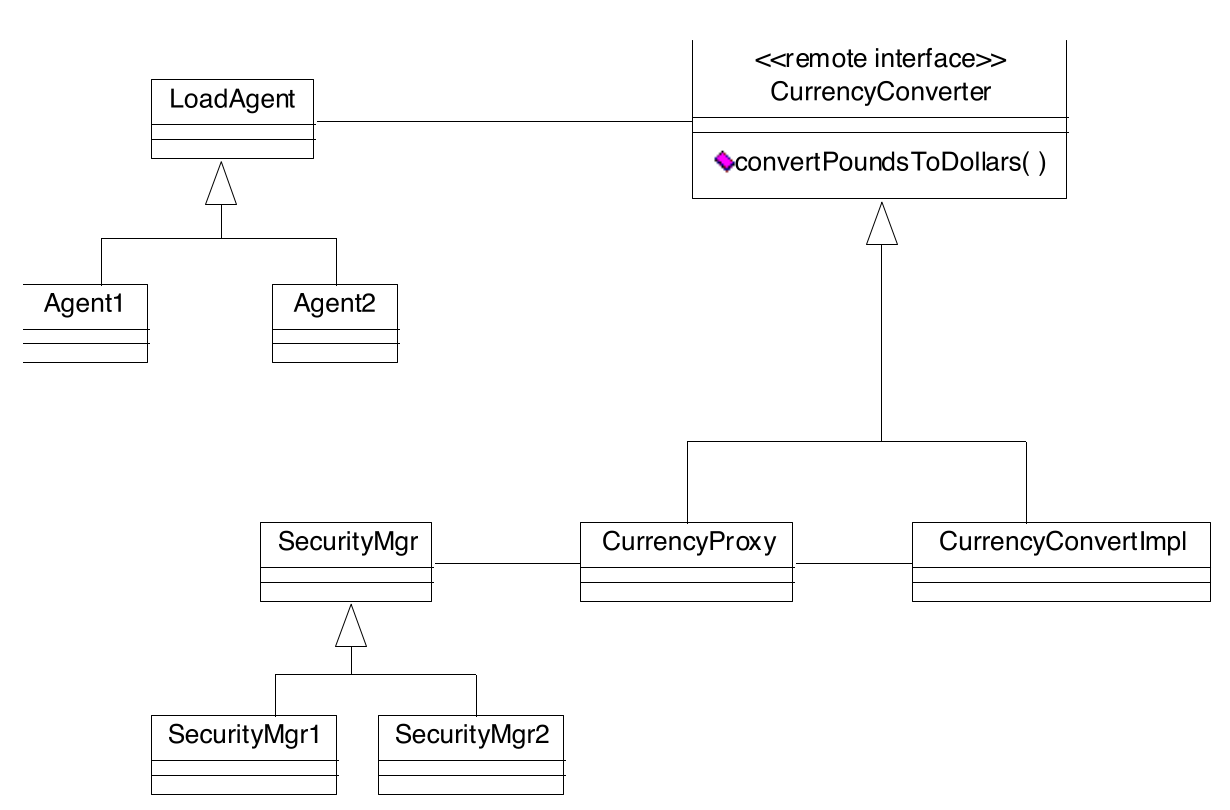
\includegraphics[width=0.7\textwidth]{./images/distributed_system_scenario.png}
    \caption{
        Business logic, distribute the object, add security manager, add load balancing agent.
    }
\end{figure}

\subsection{EJB}
\textbf{Enterprise Java Beans (EJB)} is a server-side component architecture that enables and simplifies the process of building enterprise-class distributed object applications in Java.
It allows you to write scalable, reliable, and secure applications without writing your own complex distributed object frameworks.
EJB is a \textit{specification}.

\begin{figure}[H]
    \centering
    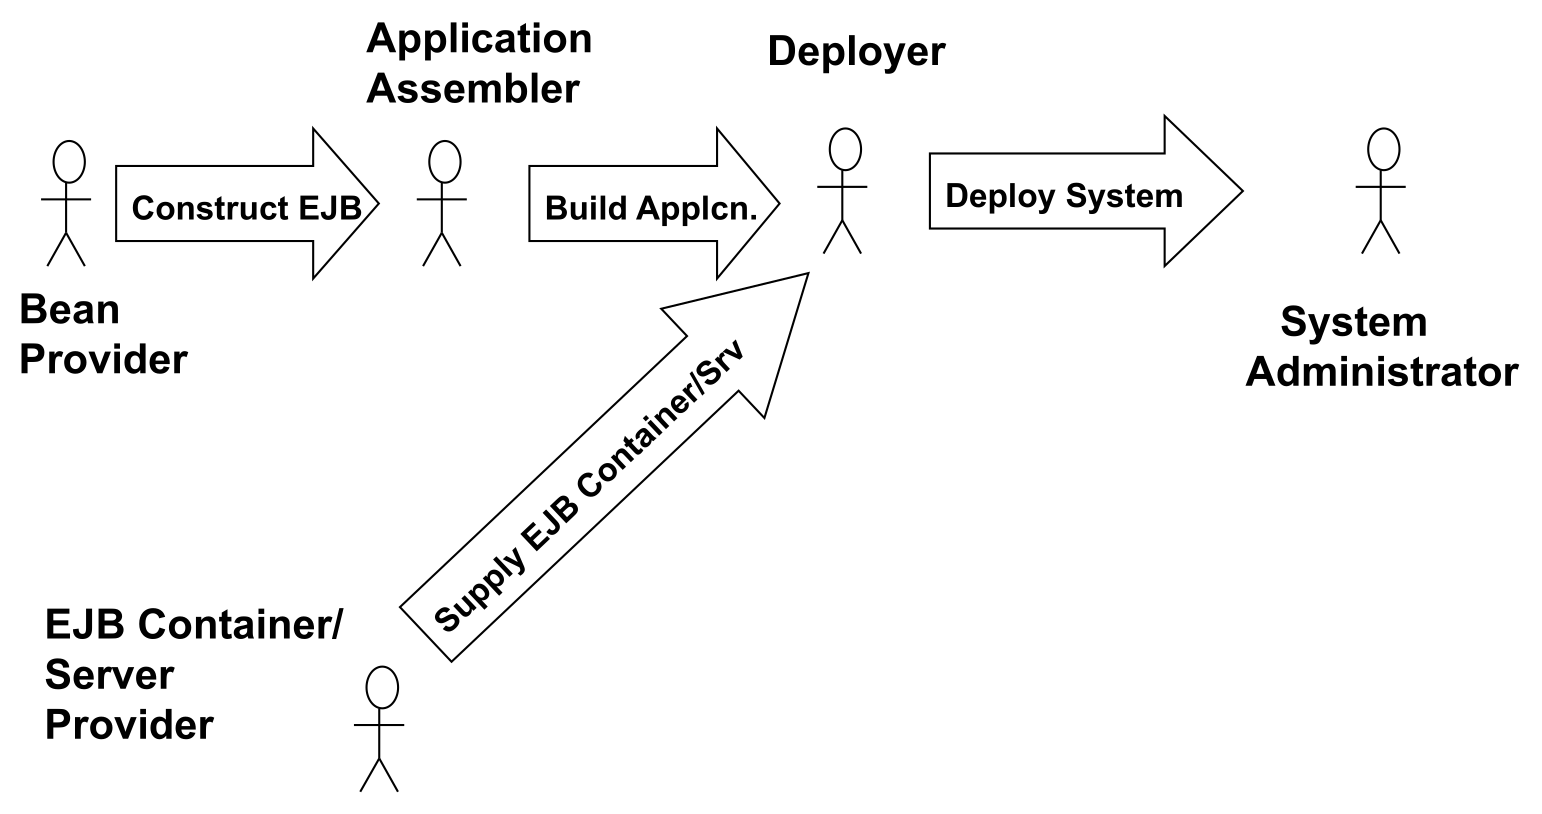
\includegraphics[width=0.7\textwidth]{./images/the_ejb_proces.png}
    \caption{
        The EJB process
    }
\end{figure}

The \textbf{EJB Container} is where the EJBs run and is responsible for managing EJBs.
The \textbf{EJB Server} is a runtime environment for container(s) that manages the low-level system resources.

\begin{figure}[H]
    \centering
    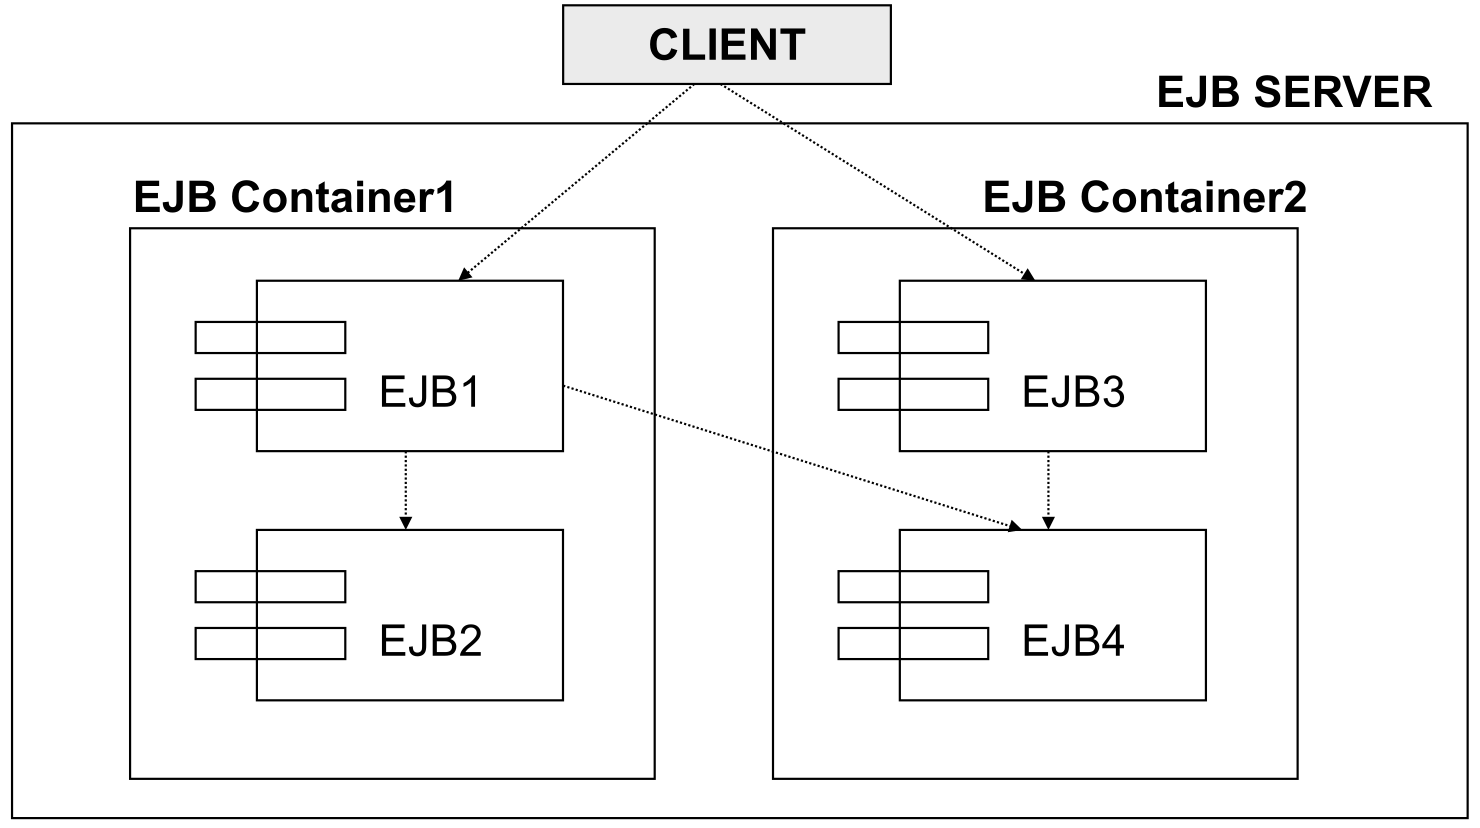
\includegraphics[width=0.7\textwidth]{./images/ejb_server_and_container.png}
    \caption{ The EJB server \& containers }
\end{figure}

\begin{figure}[H]
    \centering
    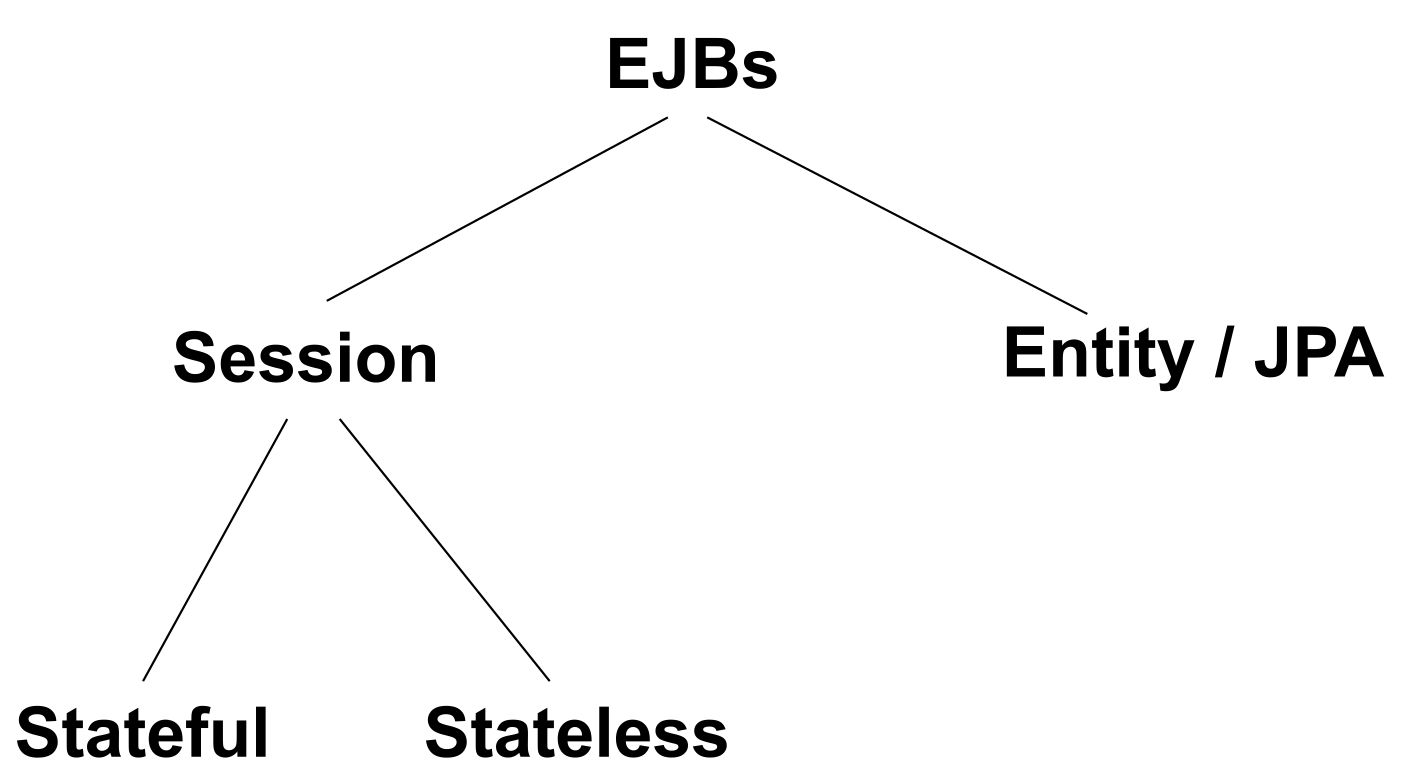
\includegraphics[width=0.7\textwidth]{./images/ejb_bean_types.png}
    \caption{ EJ Bean types }
\end{figure}

\textbf{Session beans} are ``business process objects'' (e.g., price quoting, order entry, video compression, stock trades, etc.) and live for as long as the client's session.
They are usable by 1 client at a time and are \textit{not} shared.
The EJB server manages the lifetime of beans.
\textbf{Stateless session beans} are single request with no state kept, e.g., currency converter, compression utility, or credit card verification.
\\\\
\textbf{Entity beans / JPA} represent persistent data.
They are the object-oriented in-memory view of data in an underlying data store.
They are long-lasting and have shared access.
Sub-types of entity beans include: bean-managed persisted entity beans and container-manager persistent entity beans.
\textbf{Bean-managed persistence} must be persisted manually and must look after saving, loading, \& finding.
They make use of a persistence API such as JDBC or SQL/J.
\textbf{Container-managed persistence} is automatic persistence wherein the container/server looks after the loading, saving, \& finding of component data.
You must describe what you want persisted.
Deployment tools provide support for defining simple object-relational mappings.
\\\\
The client never invokes the bean instance, instead it invokes the \textbf{EJB object} by an invocation that is intercepted by the container, delegated to the bean instance.
The EJB object is a surrogate, network-aware wrapper object that serves as a layer of indirection between the client \& the bean; it is essentially the glue between the client \& the bean.
EJB objects must clone every business method that your bean class exposes, specified in the remote interface.
All remote interfaces derive from \mintinline{java}{javax.ejb.EJBObject}.

\begin{figure}[H]
    \centering
    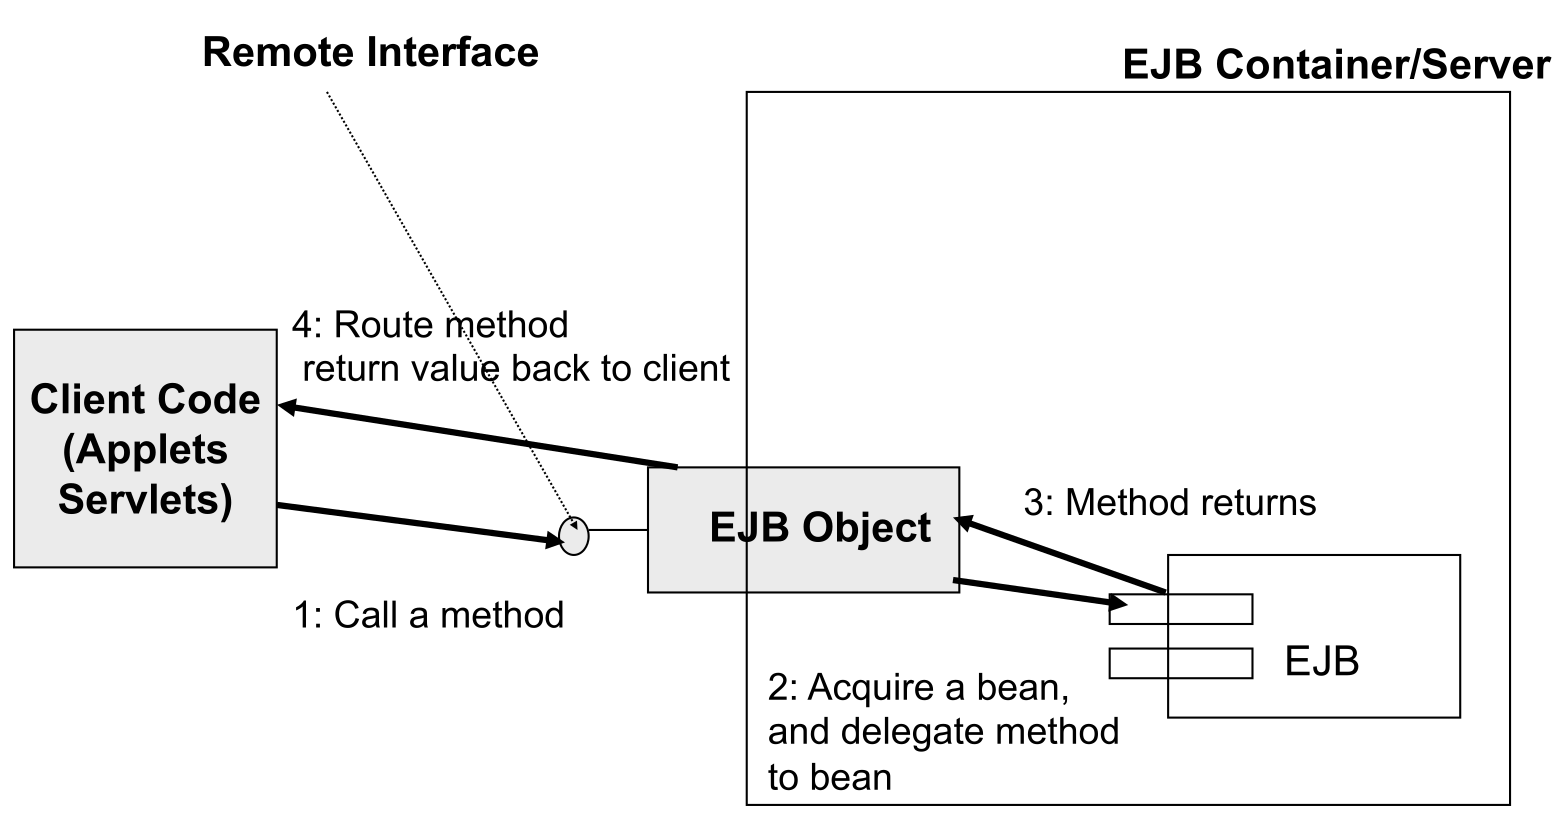
\includegraphics[width=0.7\textwidth]{./images/ejb_objets.png}
    \caption{ EJB Objects }
\end{figure}

The \textbf{session bean interface} is implemented by all session beans and specifies lifecycle methods that may be implemented inn the bean such as \mintinline{java}{setSessionContext}, \mintinline{java}{ejbCreate}, \mintinline{java}{ejbRemove}, \mintinline{java}{ejbPassivate}, \& \mintinline{java}{ejbActivate}.
\\\\
The \textbf{Java Naming \& Directory Interface} is used to find an object.
The resource (e.g., a bean) is associated with a nickname when deploying; clients of this bean can then use this nickname to look up the resource across a deployment.
The client code looks up the reference in JNDI and calls business methods on the EJB object.

\subsubsection{Entity EJBs}
\textbf{Entity EJBs} are object-based representations of information-tier data such as data stored in a relational database.
They represent a particular unit of data, e.g., a record in a database.
There are two types of entity EJB:
\begin{itemize}
    \item   Bean-managed persistence;
    \item   Container-managed persistence.
\end{itemize}

\section{NodeJS}
\textbf{NodeJS} is a JavaScript runtime environment that runs Google Chrome's V8 engine.
It is a server-side solution for JavaScript which compiles JavaScript, making it quite fast.
It was created in 2009 and designed for high concurrency, without threads or new processes.
It has evented I/O for JavaScript, and never blocks, not even for I/O.
It's goal is to provide an easy way to build scalable network programs.
It provides a JavaScript API to access the network \& file system and instead of threads, node uses an event loop with a stack which alleviates the overhead of context switching.
\begin{itemize}
    \item   JavaScript on the server-side ensures that communication between the client and the server will happen in the same language, with native JSON objects on both sides.
    \item   Servers are normally thread-based, but Node is \textbf{event-based}; Node serves each request in an evented loop that can handle simultaneous requests.
    \item   Node is a platform for writing JavaScript applications outside web browser, and is therefore not quite the same as the JavaScript we are familiar with in web browser: there is no DOM built-in to Node, nor any other browser capability.
    \item   Node doesn't run in a GUI, but runs in the terminal or as a background process.
\end{itemize}

\begin{table}[H]
    \centering
    \begin{tabular}{|p{0.5\textwidth}|p{0.5\textwidth}|}
            \hline
            \textbf{Threads} & \textbf{Event-Driven} \\
            \hline
            Lock application / request with listener-workers threads. & Only one thread, which repeatedly fetches an event. \\
            \hline
            Uses incoming-request model. & Uses queue and then process it. \\
            \hline
            Multi-threaded server might block the request which might involve multiple events. & Manually saves the state and then goes on to process the next event. \\
            \hline
            Uses context switching. & No contention and no context switches.\\
            \hline
            Uses multi-threading environments where the listener \& worker threads are used frequently to take an incoming-request lock & Uses asynchronous I/O facilities (callbacks, nor poll/select or \verb|O_NONBLOCK| environments).\\
            \hline
        \end{tabular}
    \caption{Threads versus asynchronous event-driven}
\end{table}

Ordinarily, a webserver waits for server-side I/O operations to complete while processing a web client request, thus \textbf{blocking} the next request to be processed.
Servers generally do nothing but I/O, and scripts waiting on I/O requests degrades performance.
Node processes each request as an event, it doesn't wait for the I/O operation to complete, making it \textbf{non-blocking}; it can therefore handle other requests at the same time.
When the I/O operation of the first request is completed, it will callback the server to complete the request.
To avoid blocking, Node makes use of the event-driven nature of JavaScript by attaching callbacks to I/O requests.
Scripts waiting on I/O waste no space because they get popped off the stack when their non-I/O related code finishes executing.

\subsection{MEAN}
\textbf{MEAN} is a full stack solution consisting of MongoDB, Express, Angular, \& node.

\begin{figure}[H]
    \centering
    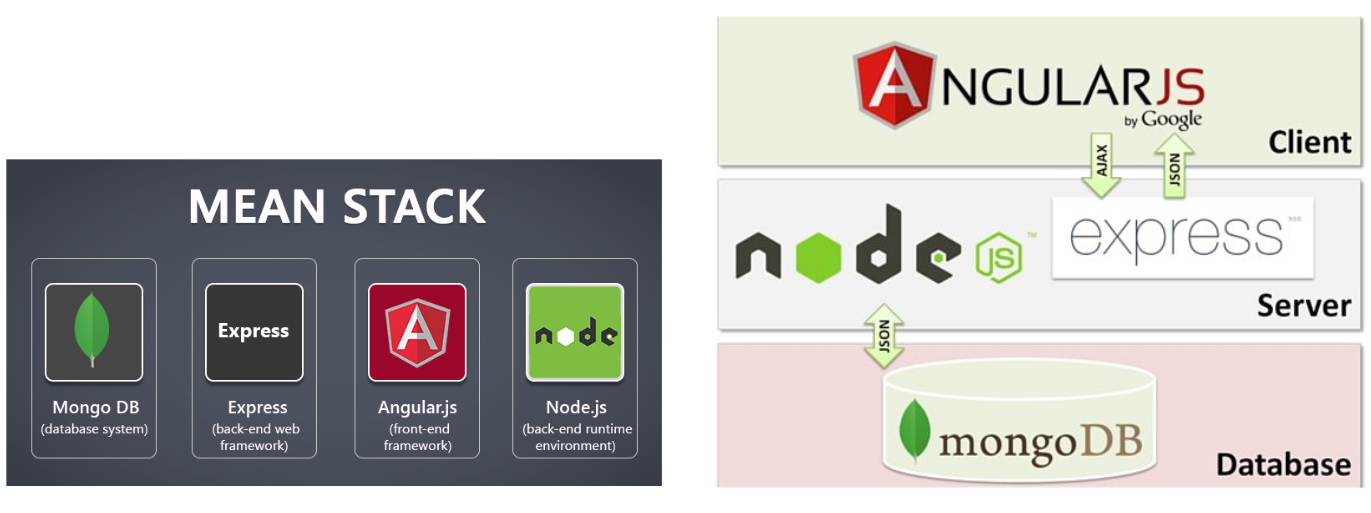
\includegraphics[width=0.7\textwidth]{./images/mean.png}
    \caption{ MEAN stack }
\end{figure}

\section{Proxmox Virtualisation Environment}
\textbf{Proxmox} is an open-source hyper-converged virtualisation environment.
It has a bare-metal installer, a web-based remote management GUI, a HA cluster stack, unified cluster storage, and a flexible network setup.
It has commercial support packages available at a reasonable cost.
Proxmox uses the following underlying technologies:
\begin{itemize}
    \item   KVM (type 1 hypervisor module for Linux).
    \item   QEMU hardware emulation.
    \item   LXC Linux containers.
    \item   Ceph replicated storage.
    \item   Corosync cluster engine.
\end{itemize}

\subsection{KVM}
\textbf{Kernel-based Virtual Machine (KVM)} is a virtualisation infrastructure for the Linux kernel that turns it into a hypervisor.
KVM requires a processor with hardware virtualisation extensions and a wide variety of guest operating systems work with KVM.
It supports a paravirtual Ethernet card, a paravirtual disk I/O controller using VitrIO, a balloon device for adjusting guest memory usage, and a VGA graphics interface.

\subsection{QEMU}
\textbf{QEMU (Quick Emulator)} is an open-source hosted hypervisor that performs hardware virtualisation.
It emulates CPUs through dynamic binary translation and provides a set of device models, enabling it to run a variety of unmodified guest operating systems.
It uses KVM Hosting mode in Proxmox where QEMU deals with the setting-up and migration of KVM images.
It is still involved in the emulation of hardware, but the execution of the guest is done by the KVM as requested by QEMU.
It uses the KVM to run virtual machines at near-native speed (requiring hardware virtualisation extensions on x86 machines).
When the target architecture is the same as the host architecture, QEMU can make use of KVM particular features, such as acceleration.

\subsection{LXC}
\textbf{LXC (Linux Containers)} is an operating-system-level virtualisation method for running multiple isolated Linux systems (containers) on a control host using a single Linux kernel.
The Linux kernel provides the cgroups (control groups) functionality that allows limitation \& prioritisation of resources (CPU, memory, block I/O, network, etc.) without the need for starting any virtual machines.
It provides namespace isolation functionality that allows complete isolation of an application's view of the operating environment, including process tress, networking, user IDs, and mounted file systems.
LXC combines the kernel's cgroups and support for isolated namespaces to provide an isolated environment for applications.
Docker can also use LXC as one of its execution drivers, enabling image management and providing deployment services.

\subsection{Ceph}
\textbf{Ceph} is a storage platform that implements object storage on a single distributed computer cluster, and provides interfaces for object-level, block-level, \& file-level storage.
Ceph aims for completely distributed operation without a single point of failure, scalable to the exabyte level.
Ceph's software libraries provide client applications with direct access to the Reliable Autonomic Distributed Object Store (RADOS) object-based storage system.
Ceph replicates data and makes it fault-tolerant, using commodity hardware and requiring no specific hardware support.
As a result of its design, the system is both self-healing and self-managing, aiming to minimise administration time and other costs.
When an application writes data to Ceph using a block device, Ceph automatically striped and replicates the data across the cluster.
It works well with the KVM.

\begin{figure}[H]
    \centering
    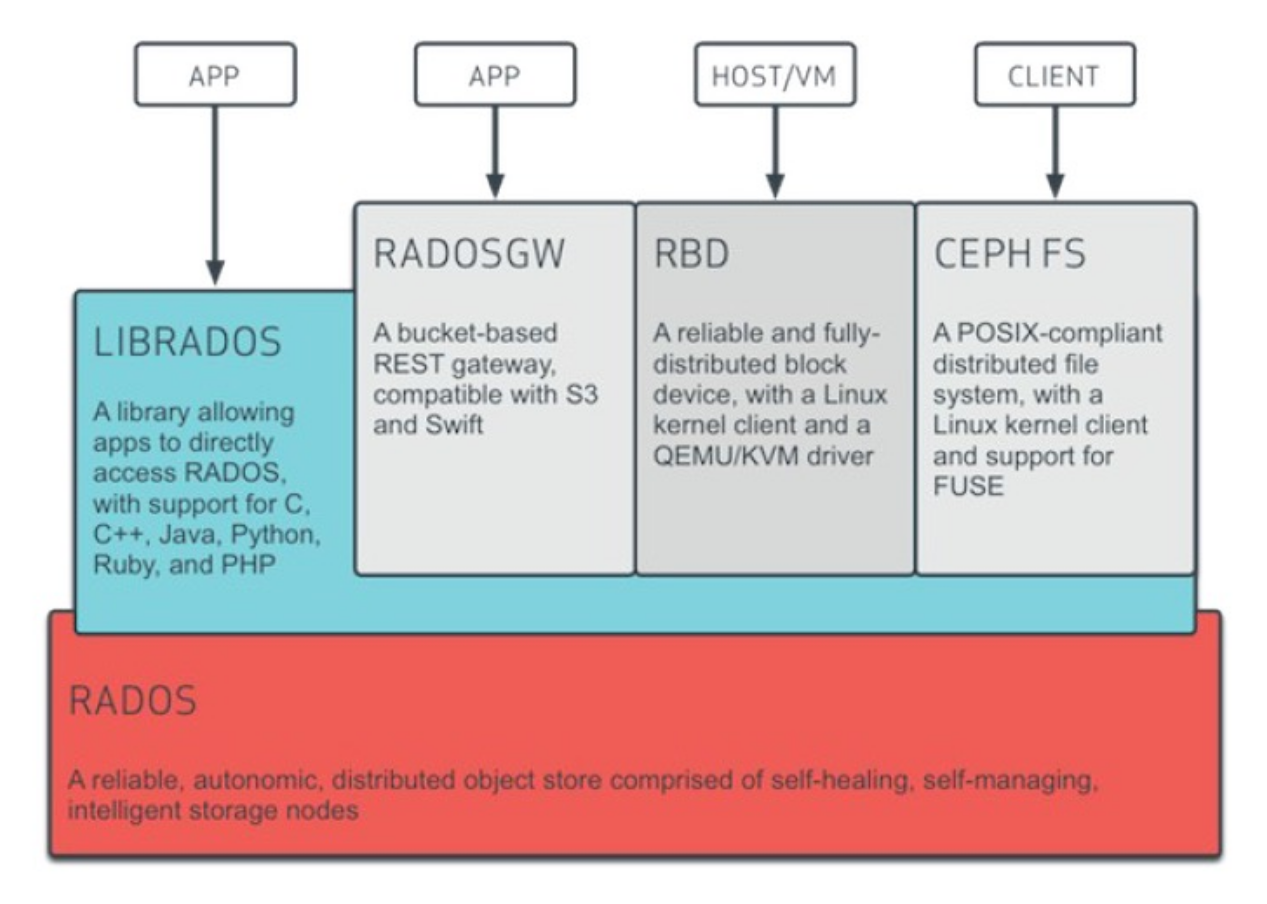
\includegraphics[width=0.7\textwidth]{./images/ceph.png}
    \caption{ Ceph architecture }
\end{figure}

\begin{figure}[H]
    \centering
    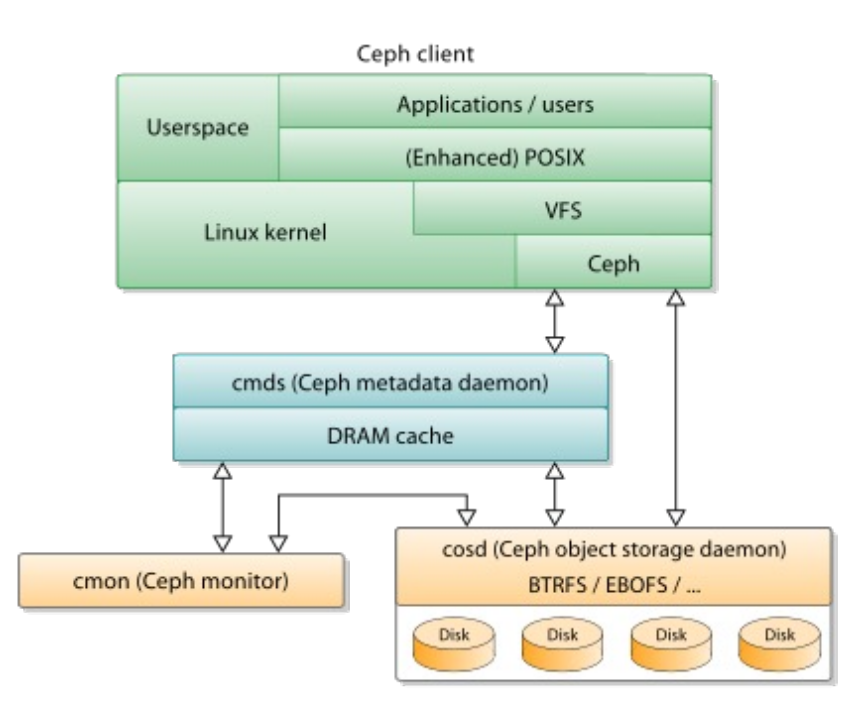
\includegraphics[width=0.7\textwidth]{./images/cephinternal.png}
    \caption{ Ceph internal organisation }
\end{figure}

\subsubsection{Ceph Network}
To create a Ceph \verb|ring0| network, each node must be reachable on \verb|rin0|.
The firewalls on each node will need to be checked to verify this.
Proxmox distribute their own Ceph package as of version 5.1:
\begin{itemize}
    \item   \verb|pveceph install| will install the latest stable repositories \& packages -- must be run on each node individually.
    \item   \verb|ceph init --network x.x.x.x/y| must be run on the first node only.
    \item   \verb|ceph createmon| must be ran on each node.
\end{itemize}

\subsubsection{Ceph OSDs}
We can add disks as \textbf{Object Storage Devices (OSD)s} on each node.
The accurate network time is also very important to avoid ``clock skew''.
The latest network time system daemon \verb|system.time?| is much better than \verb|ntpdate|.
QEMU has a new time source driver which can be run in guests needing accurate time.
\\\\
\textbf{Pools} are individual storage blocks:
\begin{itemize}
    \item   \verb|size| is the number of replications (OSDs) per block.
    \item   \verb|min-size| is the minimum number of OSDs (replications) each block must be on to allow read-write status.
    \item   \verb|add-storage| option automatically adds the storage block to the hosts rather than having to manually copy the Ceph keys to each host to allocate the storage.
\end{itemize}

The client (Proxmox) interacts with one OSD only.
This OSD then write to and confirms write on each OSD in the block before confirming write completion.
Writes are actually made to the journal rather than the block level device for speed.
This primary OSD manages all interactions with both the client and the replication OSDs.
In case the primary manager is lost, a backup OSD will take over as primary.
\\\\
\textbf{Crush maps} define the actual storage blocks (these are very complicated so don't change the default settings!).
As new OSDs are added, Ceph will attempt to re-allocate data across blocks to improve access \& availability.
If an OSD gets removed, Ceph will rebalance data once the OSD is marked as OUT (300 seconds by default).
Use \verb|ceph noout| to avoid rebalancing, e.g., for maintenance.

\subsection{VM Installation}
\subsubsection{Hard Drives}
For hard drives, \verb|virtio-scsi| and \verb|scsi| are the best-performance options.
On Windows VMs, this can be a chore as it is necessary to use a second boot CD to install \verb|virtio| drivers.
No-cache is the best compromise option for local disks, as the write-back is the fastest, although it is unsafe on Ceph.

\subsubsection{Memory}
Fixed allocation with ballooning is the best way to allocate RAM.
Over-provisioning is possible but dangerous as guests may crash if RAM is not available.
Auto-allocation of memory means that required RAM may take up to 30 seconds to be available;
it is best to leave swap enabled as this way, swap is a last option before crashing.

\subsubsection{VM Backups}
There are two types of backup types:
\begin{itemize}
    \item   \textbf{Snapshot} leaves the guest running and intercepts all write operations, writes them to the backup if the block is already backed up, then to the guest.
            This slows the guest I/O down to the speed of the backup medium.
    \item   \textbf{Stop} causes the guest to shutdown, then restarts and does backup before making the guest available.
\end{itemize}

\subsubsection{VM Migration}
For guests on local storage, migration must done offline.
Any storage used in the guest (e.g., ZFS) must be available on the target node.
guests can be live moved to shared storage (e.g., NFS or Ceph) and then live migrated.

\subsubsection{VM Cloning}
\textbf{Linked clones} allow the fast spin-up of machines as only diverging blocks need to be written to the disk.
Linked clones require file-level storage system, i.e., snapshot-able storage.
The conversion of a VM to a template sets the image as read-only.

\subsubsection{VM Imports}
To perform \textbf{OVA import}, first unpack the OVA, for example onto a NAS.
Then run \verb|qm help importovf| for details of the import command.
To perform \textbf{disk import}, run \verb|qm help importdisk|.
\verb|vmdebootstrap| can be used to build Debian disk images programmatically.
\verb|qm help create| can be ran for details on creating VMs programmatically.
\\\\
Note that Windows disk images will not have any \verb|virtio| drivers installed by default:
the hard disk types must be SATA, the network devices must be E1000.
Spice-space spice-guest-tools can be used to install all \verb|virtio| drivers into Windows images.
The Spice repository on GitHub has the source code for the installation tools.

\subsubsection{User Authentication}
\textbf{PAM authentication} can be used for per-machine authentication (may be possible to integrate radius).
\textbf{Proxmox authentication server} replicates authentication across all nodes.

\subsection{Proxmox Cluster}
The \textbf{Proxmox VE cluster manager \texttt{pvecm}} is a tool to create a group of physical servers called a \textbf{cluster}.
It uses the Corosync Cluster Enginer for reliable group communicaiton, and such clusters can consist of up to 32 physical nodes or more, dependent on the network latency (must be less than 2 milliseconds).
\verb|pvecm| can be used to create a new cluster, join nodes to a cluster, leave the cluster, get status information, and do various other cluster-related tasks.
\\\\
Grouping Proxmox hosts into a cluster has the following advantages:
\begin{itemize}
    \item   Centralised, web-based management of a multi-master cluster: each node can do all management tasks.
    \item   \verb|pmxcfs|: a database-driven file system for storing configuration files, replicated in real-time on all nodes using the corosync cluster engine.
    \item   Migration of VMs \& containers between physical hosts.
    \item   Fast deployment \& cluster-wide services like firewall and High Availability (HA).
\end{itemize}

\subsection{High Availability}
Items managed under HA are referred to as \textit{resources}:
\begin{itemize}
    \item   The HA cluster is managed by \verb|pve-ha-crm.service|.
    \item   The local HA resources are managed by \verb|pve-ha-lrm.service|.
\end{itemize}

The Guest HA is managed either through the dropdown on the guest window, or HA options on the Datacenter and this allows a guest VM to be automatically migrated or restarted on a different node if it is detected as down, e.g., because of node failure or maintenance.
\\\\\
Ensure that \verb|pve-ha-crm| and \verb|pve-ha-lrm| are both running under \verb|node -> services|.
All migrations and other actions on HA resources are managed by the HA daemon.
The task viewer only shows status of the request to HA daemon to carry out the task, not of the actual task.
\\\\
Migrations (generally, but particularly under HA conditions) may fail due to a number of causes, including:
\begin{itemize}
    \item   The guest has local attached storage which is not available on the target node.
    \item   The guest has NUMA (Non-Uniform Memory Access) or other CPU settings not present on the target node.
\end{itemize}

Changing the HA manager state for a VM will cause the VM state to change.
If any node hosting a HA resource loses corosync quorum:
\begin{enumerate}
    \item   The \verb|pve-ha-lrm.service| will no longer be able to write to the watchdog timer service.
    \item   After 60 seconds, the node will reboot.
    \item   After a further 60 seconds, the VM will be brought up on a different node.
\end{enumerate}

\subsubsection{HA Groups}
Group members will prefer selected nodes if available:
\begin{itemize}
    \item   If \verb|restricted| is selected, members will only run on selected nodes.
    \item   Guests will be stopped by the HA manager if the node(s) become unavailable.
    \item   If \verb|nofailback| is not selected, guests will try to migrate back to a preferred node once it becomes available again.
\end{itemize}

\subsection{Performance Benchmarking}
\begin{itemize}
    \item   \verb|iperf| to test network throughput.
    \item   \verb|systat| to monitor system statistics.
    \item   \verb|iostat| to test I/O throughput.
\end{itemize}























\end{document}
